\section{ERM}


Ein \acrfull{ERM} ist eine abstrakte Darstellung der Tabellen (Entities), die in einer Datenbank angelegt sind, sowie der Beziehungen (Relationships) zwischen den Tabellen. Jede Tabelle kann mehrere Kolonnen (=Attribute) haben.

Wenn man eine Datenbank erstellt, kann es nützlich sein, zuerst ein \gls{ERM} aufzuzeichnen, um sich zu überlegen, welche Tabellen es braucht.

Das \gls{ERM} des sozialen Netzwerks InstaHub ist in \cref{fig:erm-instahub} abgebildet. \cref{fig:erm-components} zeigt die Darstellung der Komponenten eines ERM in der sogenannten Chen-Notation.

\begin{figure}[H]
  \centering
  \begin{tikzpicture}[auto]
    % Nodes
    \node[entity] (user) at (0,0) {users};
    \node[relationship] (follows) at (-4,0) {follows};
    \node[relationship] (owns) at (2.5,2.5) {owns};
    \node[entity] (photo) at (5,0) {photos};
    \node[relationship] (has) at (7,0) {has};ff
    \node[entity] (tag) at (9,0) {tags};
    \node[relationship] (comments) at (2.5,0) {comments};
    \node[relationship] (likes) at (2.5,-2.5) {likes};
    \node[relationship] (haspw) at (0,-2) {has};
    \node[entity] (pwreset) at (-4,-2) {password\_resets};

    % Edges
    \draw (user) -- (follows) node[midway, above] {m};
    \draw (follows) -- (user) node[midway, below] {n};
    \draw (user) -- (owns) node[midway, above] {1};
    \draw (owns) -- (photo) node[midway, above] {n};
    \draw (photo) -- (has) node[midway, above] {n};
    \draw (has) -- (tag) node[midway, above] {m};
    \draw (user) -- (comments) node[midway, above] {n};
    \draw (comments) -- (photo) node[midway, above] {m};
    \draw (user) -- (likes) node[midway, left] {n};
    \draw (likes) -- (photo) node[midway, right] {m};
    \draw (user) -- (haspw) node[midway, left] {1};
    \draw (haspw) -- (pwreset) node[midway, above] {n};
  \end{tikzpicture}
  \caption{\gls{ERM} von InstaHub}
  \label{fig:erm-instahub}
\end{figure}

\begin{figure}[H]
  \centering
  \begin{tikzpicture}[node distance=1cm]

    % Entity
    \node[entity] (entity1) {Entity};
    \node[attribute] (attr1) [above left=of entity1] {Attribute} edge (entity1);
    \node[attribute] (attr2) [below left=of entity1] {Attribute} edge (entity1);

    % Relationship
    \node[relationship] (rel1) [right=3cm of entity1] {Relationship} edge node[auto,swap] {n} (entity1);
    \node[entity] (entity2) [right=3cm of rel1] {Entity} edge node[auto,swap] {m} (rel1);
    \node[attribute] (attr3) [above=of rel1] {Attribute} edge (rel1);

    % Legend
    \node[draw,thick,fit=(entity1) (attr1) (attr2),inner sep=0.5cm, rounded corners, dotted, red] (box1) {};
    \node[anchor=south, red] at (box1.north) {Tabellen (\textit{Entities}) und Attribute};

    \node[draw,thick,fit=(rel1) (entity2) (attr3),inner sep=0.5cm, rounded corners, dotted, blue] (box2) {};
    \node[anchor=south, blue] at (box2.north) {Beziehungen (\textit{Relationships})};

  \end{tikzpicture}
  \caption{\gls{ERM}-Komponenten in der sogenannten Chen-Notation}
  \label{fig:erm-components}
\end{figure}

Die \textit{entities}, die meistens einer Tabelle entsprechen, werden als Rechtecke angegeben. Beziehungen stellen ``Verknüpfungen'' zwischen verschiedenen Tabellen dar und sind meist als Raute dargestellt. Die Attribute werden typischerweise als Kreise angegeben. In \cref{fig:erm-instahub} sind die Attribute einfachheitshalber nicht angegeben.

Die Zahlen über den Strichen bezeichnen die \textbf{Kardinalität} der Beziehungen: Mit der Kardinalität wird ausgedrückt, wie viele Entitäten mit einer anderen Entität in Verbindung stehen können oder müssen:
\begin{itemize}
  \item \textbf{Eins-zu-Eins (1:1)}: Dies wird normalerweise angezeigt, indem eine ``1'' in der Nähe beider Entitäten platziert wird, die durch eine Beziehung verbunden sind. Es bedeutet, dass eine Instanz einer Entität mit genau einer Instanz einer anderen Entität assoziiert ist.
  \item \textbf{Eins-zu-Viele (1:n)}: Dies wird dargestellt, indem eine ``1'' in der Nähe der Entität auf der 'eins'-Seite der Beziehung und ein ``n'' oder ``m'' (für ``\textit{many}''=viele) in der Nähe der Entität auf der ``viele''-Seite der Beziehung platziert wird. Es zeigt an, dass eine Instanz der ersten Entität mit null, einer oder mehreren Instanzen der zweiten Entität assoziiert sein kann, aber eine Instanz der zweiten Entität nur mit einer Instanz der ersten Entität assoziiert sein kann.
  \item \textbf{Viele-zu-Viele (m:n)}: Dies wird gezeigt, indem ein ``m'' oder ``n'' in der Nähe beider Entitäten platziert wird. Es zeigt an, dass Instanzen der ersten Entität mit null, einer oder mehreren Instanzen der zweiten Entität assoziiert sein können und umgekehrt.
\end{itemize}

Folgende Fakten können beispielsweise am \gls{ERM} in \cref{fig:erm-instahub} abgelesen werden:
\begin{itemize}
  \item Jeder \texttt{user} kann beliebig viele (oder 0) \texttt{comments} schreiben.
  \item Jeder \texttt{user} kann beliebig vielen (oder 0) anderen Usern followen und kann von beliebig vielen (oder 0) andern usern gefollowt werden.
  \item Jedes Foto kann beliebig viele (oder 0) Tags haben. Jeder Tag kann auf \texttt{n} Fotos angewandt werden.
  \item Jedes Fotos gehört genau zu einem Benutzerprofil (\texttt{owns}). Jedes Benutzerprofil kann beliebig viele (oder 0) Fotos veröffentlichen.
  \item Jeder \texttt{user} kann sein Passwort beliebig viele male (oder 0 mal) zurückgesetzt haben. Jedes des \texttt{password\_resets} kann aber nur einen \texttt{user} betreffen.
\end{itemize}


\begin{myexercise}
  Eine Schule möchte ihre Datenbankstruktur neu organisieren, um Informationen über Lehrer, Schüler und Klassen besser verwalten zu können.
  Die Schule hat entschieden, ein Entity-Relationship-Modell (ERM) zu entwerfen, um die Beziehungen zwischen diesen Entitäten klar darzustellen (s. \cref{fig:erm-school}).
  Was fällt Ihnen in diesem \gls{ERM} auf? Stimmen die Kardinalitäten?
  \begin{figure}[H]
    \centering
    \resizebox{\textwidth}{!}{%
      \begin{tikzpicture}
        % Entitäten
        \node[entity] (lehrer) at (0,0) {Lehrer};
        \node[entity] (schueler) at (14,0) {Schüler};
        \node[entity] (klasse) at (7,0) {Klasse};

        % Beziehungen
        \node[relationship] (unterrichtet) at (3.5,0) {unterrichtet};
        \node[relationship] (gehoert_zu) at (10.5,0) {gehört zu};

        % Kanten
        \draw (lehrer) -- (unterrichtet) node[midway,above]{n};
        \draw (unterrichtet) -- (klasse) node[midway,above]{0:1};
        \draw (schueler) -- (gehoert_zu) node[midway,above]{1};
        \draw (gehoert_zu) -- (klasse) node[midway,above]{m};
      \end{tikzpicture}
    }

    \caption{\gls{ERM} einer Schul-Datenbank}
    \label{fig:erm-school}
  \end{figure}

  \begin{myanswer}
    Ein Lehrer kann in diesem \gls{ERM} nur 0 oder 1 Klasse unterrichten. 
    In Realität ergibt es keinen Sinn, dass ein Lehrer keine Klasse unterrichtet, und auch die Beschränkung auf maximal eine Klasse ergibt keinen Sinn.
    Statt \texttt{0:1} sollte also \texttt{m} stehen zwischen ``unterrichtet'' und ``Klasse''. 
Zudem sollten \texttt{m} und \texttt{1} zwischen \textit{Klasse} und \textit{Schüler} getauscht werden.
  \end{myanswer}
\end{myexercise}

\begin{myexercise}
  Ein Krankenhaus möchte seine Datenbankstruktur neu organisieren, um Informationen über Ärzte, Patienten und Behandlungen effizienter zu verwalten. Das Krankenhaus hat sich entschieden, ein Entity-Relationship-Modell (ERM) zu entwerfen, um die Beziehungen zwischen diesen Entitäten klar darzustellen (s. \cref{fig:erm-hospital}).
  \begin{figure}[H]
    \centering
    \begin{tikzpicture}
      % Entitäten
      \node[entity] (aerzte) at (0,0) {Ärzte};
      \node[entity] (patienten) at (0,-3) {Patienten};
      \node[entity] (behandlungen) at (7,-1.5) {Behandlungen};

      % Beziehungen
      \node[relationship] (behandelt) at (2.5,-1.5) {behandelt};

      % Kanten
      \draw (aerzte) -- (behandelt) node[midway,above]{n};
      \draw (behandelt) -- (behandlungen) node[midway,above]{m};
      \draw (patienten) -- (behandelt) node[midway,below]{1};

    \end{tikzpicture}
    \caption{ERM eines Krankenhaus-Datenbanksystems}
    \label{fig:erm-hospital}
  \end{figure}
  Bewerten Sie das dargestellte ERM. Sind die Kardinalitäten korrekt angegeben?
  \begin{myanswer}
    In dem dargestellten ERM wird angenommen, dass ein Arzt mehrere Behandlungen durchführen kann (n:m-Beziehung) und dass jeder Patient genau eine Behandlung erhält (1:m-Beziehung). Diese Annahme ist jedoch nicht ganz realistisch, da ein Patient mehrere Behandlungen erhalten könnte. Die Kardinalität zwischen ``Patienten'' und ``behandelt'' sollte daher m sein, um anzugeben, dass ein Patient mehrere Behandlungen erhalten kann.
  \end{myanswer}
\end{myexercise}


\clearpage


\section{Informationen aus mehrere Tabellen kombinieren}
\subsection{Primärschlüssel}
Wie in \cref{subsec:tables} diskutiert wurde, besitzen Tabellen häufig sogenannte Primärschlüssel (en. \textit{primary keys}). \cref{table:angestellte} beispielsweise verwendet einen Primärschlüssel \underline{mID} (blaue Kolonne, hervorgehoben mit dem Symbol \emoji{key}). 

\begin{table}[H]
\centering
\begin{tabular}{a|l|l}
\emoji{key} \underline{mID} & Name   & ... \\\midrule
1  & Müller  & ...  \\
2  & Schmidt & ...  \\
3  & Kaufmann  & ...\\
... & ... & ... 
\end{tabular}
\caption{Beispiel-Tabelle: ``Angestellte''}
\label{table:angestellte}
\end{table}

Dieser dient in erster Linie dazu, einen Eintrag (in diesem Fall eine Person) eindeutig zu identifizieren. Weshalb ist das nötig? 

Zwei Hauptgründe seine angegeben:

\begin{itemize}
\item \textbf{Eindeutigkeit}: Es könnte sein, dass zwei Personen gleich heissen. In diesem Fall ist es hilfreich, eine eindeutige Identifikationsnummer (oder einen eindeutigen Text) zu haben, um Information zu genau \textit{einer} der beiden Personen abfragen zu können.
\item \textbf{Dauerhaftigkeit}: Es könnte sein, dass eine Person den Namen wechselt. In diesem Fall möchte man eine eindeutige Identifikationsnummer haben, damit die Informationen zu den Personen wie etwa der Gehalt oder die Abteilung weiterhin eindeutig zur selben Person gehören (und abgefragt werden können).
\end{itemize}

\subsection{Fremdschlüssel}
Nebst Primärschlüsseln können Tabellen auch sogenannte Fremdschlüssel (en. \textit{foreign keys}) besitzen, die sich auf Primärschlüssel von anderen Tabellen beziehen. Dies erlaubt, Informationen aus mehreren Tabellen zu kombinieren. Gegeben sei folgendes Beispiel mit je einer Tabellen zu Angestellten und Abteilungen (\cref{table:angestellte2}, \cref{table:abteilungen}).

\begin{minipage}{.48\textwidth}
\centering

\begin{table}[H]
\centering
\begin{tabular}{l|l|a}
\emoji{key} \underline{mID} & Name   & \tikzmarknode{fkey}{\underline{aID} \faKey} \\\midrule
1  & Müller  & \tikzmarknode{31o}{31}  \\
2  & Schmidt & \tikzmarknode{32o1}{32}  \\
3  & Kaufmann  & \tikzmarknode{32o2}{32}\\
... & ... & ... 
\end{tabular}
\caption{Tabelle ``\textbf{Angestellte}''}
\label{table:angestellte2}
\end{table}
\end{minipage}
\begin{minipage}{.48\textwidth}
\centering
\begin{table}[H]
\centering
\begin{tabular}{a|l}
\tikzmarknode{pkey}{\emoji{key} \underline{aID}} & Abteilung \\\midrule
\tikzmarknode{31t}{31}    & Verkauf   \\
\tikzmarknode{32t}{32}    & Technik   \\
\tikzmarknode{33t}{33}    & Marketing \\
... & ... 
\end{tabular}
\begin{tikzpicture}[overlay,remember picture]
% title
 \draw[red,-stealth] (fkey) to[bend left] (pkey);
% values
  \draw[red,-stealth] (31o) -- (31t);
  \draw[red,-stealth] (32o1) -- (32t);
  \draw[red,-stealth] (32o2) -- (32t);
\end{tikzpicture}
\caption{Tabelle ``\textbf{Abteilungen}''}
\label{table:abteilungen}
\end{table}
\end{minipage}

In diesem Beispiel hat die Tabelle ``Angestellte'' nicht nur einen Primärschlüssel \texttt{mID}, sondern auch einen Fremdschlüssel \texttt{aID} (hervorgehoben mit dem Symbol \faKey), der auf den Primärschlüssel mit demselben Name der Tabelle ``Abteilungen'' verweist. Angenommen wir möchten nun (mit SQL, nicht mit manuellem Nachschauen) herausfinden, in welcher Abteilung die Person ``Kaufmann'' arbeitet, wie lassen sich nun die Informationen aus beiden Tabellen kombinieren?



\subsection{\texorpdfstring{Tabellen verbinden mit oder ohne \lstinline[style=SQL]|JOIN|}{Tabellen verbinden mit oder ohne JOIN}}

\begin{myexample}
Eine erste Möglichkeit, \cref{table:angestellte2} mit \cref{table:abteilungen} zu verbinden, besteht darin, einfach beide Tabellen ``aufzurufen'':
\begin{lstlisting}[style=sql]
SELECT *
FROM Angestellte, Abteilung
\end{lstlisting}

\begin{table}[H]
\centering
\begin{tabular}{l|l|a|a|l}
mID & Name   &  \rot{Angestellte.aID} & \rot{Abteilung.aID} & Abteilung \\\midrule
1  & Müller  & 31  & 31  & Verkauf\\
1  & Müller  & 31  & 32  & Technik\\
1  & Müller  & 31  &33  &  Marketing\\
1  & Müller  & 31  & ...  & ...\\
2  & Schmidt & 32 &31 & Verkauf\\
2  & Schmidt & 32 &32 & Technik\\
2  & Schmidt & 32 &33 & Marketing\\
2  & Schmidt & 32 &... & ...\\
3  & Kaufmann  & 31 &... & ... \\
... & ... & ... & ... & ... 
\end{tabular}
\end{table}

Wie wir sehen, wurden Informationen aus beiden Tabellen zusammengeführt, indem alle möglichen Kombinationen beider Tabellen erstellt wurden. Die beiden gleichnamigen Kolonnen erhalten zusätzlich einen Präfix (vorausgehender Text) mit dem Namen der Ursprungstabelle, um diese voneinander abzugrenzen. 
\end{myexample}

\begin{myexample}
Wir könnten nun die Auswahl einfach eingrenzen, indem wir zwei Filter einfügen:

\begin{lstlisting}[style=sql]
SELECT *
FROM Angestellte, Abteilung
WHERE Angestellte.aID = Abteilung.aID
AND Name = "Kaufmann"
\end{lstlisting}

\begin{table}[H]
\centering
\begin{tabular}{l|l|a|a|l}
mID & Name   & \rot{Angestellte.aID} & \rot{Abteilung.aID} & Abteilung \\\midrule
3  & Kaufmann  & 32 &32 & Technik \\
\end{tabular}
\end{table}
\end{myexample}

\begin{myremark}
Bisher haben wir immer auf Kolonnen von Tabellen zugegriffen, indem wir den Namen der Kolonne geschrieben haben. Wenn wir mit mehreren Tabellen arbeiten, kann es aber passieren, dass Kolonnen denselben Namen haben. Es kann daher nötig sein, zusätzlich zum Kolonnennamen den Namen der Tabelle anzugeben.
\end{myremark}

Die Tatsache, dass unsere Abfrage mehrere Kolonnen \texttt{aID} zurückgibt, mag etwas unschön sein. Dies könnte umgangen werden, indem wir ein \lstinline[style=sql]|JOIN ... USING|-Konstrukt verwenden.
\begin{myexample} Folgender Befehl führt zu einer einzigen Kolonne \texttt{aID} im Endresultat:

\begin{lstlisting}[style=sql]
SELECT *
FROM Angestellte JOIN Abteilung USING (aID)
WHERE Name = "Kaufmann"
\end{lstlisting}

\begin{mycaution}
Die Klammer um \texttt{aID} muss gesetzt werden, damit der \lstinline[style=sql]|USING|-Befehl funktioniert.
\end{mycaution}


\begin{table}[H]
\centering
\begin{tabular}{l|l|a|l}
mID & Name   & aID & Abteilung \\\midrule
3  & Kaufmann  & 32  & Technik \\
\end{tabular}
\end{table}

\end{myexample}

\begin{myremark}
Statt zwei Tabellen können auch drei oder mehr Tabellen nach den oben erklärten Prinzipien miteinander verbunden werden. Folgendes Beispiel soll Ihnen eine Idee davon geben:

\begin{lstlisting}[style=sql]
SELECT kolonne1, kolonne2, ...
FROM tabelle1 
JOIN tabelle2 USING (kolonne_id1)
JOIN tabelle3 USING (kolonne_id2)
...
\end{lstlisting}
\end{myremark}

\begin{myremark}
Nach einer Tabellenverbindung können Sie alles machen, was Sie sonst auch tun: filtern mit \lstinline[style=sql]|WHERE|, gruppieren mit \lstinline[style=sql]|GROUP BY|, summieren mit \lstinline[style=sql]|SUM| etc.
\end{myremark}


\begin{myexercise}
Lösen Sie Aufgaben 1--10 unter folgendem Link:\\
\url{https://sql-tutorial.de/home/uebungen.php?lektion=3}.
\end{myexercise}

\section{\texorpdfstring{\lstinline[style=sql]|JOIN|-Typen}{JOIN-Typen}}


Häufig kann es nützlich sein, mehrere Tabellen auf unterschiedliche Arten miteinander zu verbinden, um neue Einsichten in die Daten zu gewinnen. Verschiedene Tabellen-Verbindungen sind schematisch in \cref{fig:venn-joins} abgebildet. Die Bedeutung dieser Abbildungen wird in den folgenden Abschnitten erklärt.


\begin{figure}[htbp]
  \centering

  % INNER JOIN
  \begin{subfigure}[b]{0.45\textwidth}
    \centering
    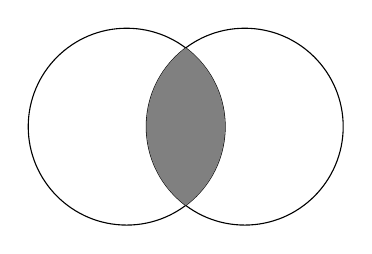
\begin{tikzpicture}
      \tikzset{circle node/.style={circle,draw=black, fill=none, minimum size=25mm, inner sep=0pt}}
      \node[circle node] (left) at (0,0) {};
      \node[circle node] (right) at (1.5,0) {};
      \begin{scope}
        \clip (0,0) circle (1.25cm);
        \fill[gray] (1.5,0) circle (1.25cm);
      \end{scope}
    \end{tikzpicture}
    \caption{\lstinline[style=sql]|INNER JOIN|}
  \end{subfigure}
  \hfill
  % LEFT OUTER JOIN
  \begin{subfigure}[b]{0.45\textwidth}
    \centering
    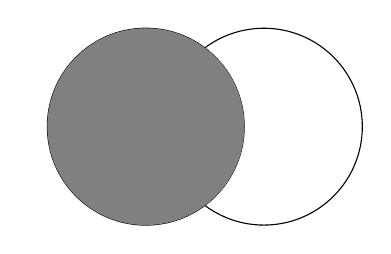
\begin{tikzpicture}
      \tikzset{circle node/.style={circle,draw=black, fill=none, minimum size=25mm, inner sep=0pt}}
      \node[circle node] (left) at (0,0) {};
      \node[circle node] (right) at (1.5,0) {};
      \begin{scope}
        \clip (-1.5,-1.25) rectangle (1.25,1.25);
        \fill[gray] (0,0) circle (1.25cm);
      \end{scope}
      \begin{scope}
        \clip (0,0) circle (1.25cm);
        \fill[gray] (1.5,0) circle (1.25cm);
      \end{scope}
    \end{tikzpicture}
    \caption{\lstinline[style=sql]|LEFT OUTER JOIN|}
  \end{subfigure}

  \bigskip

  % RIGHT OUTER JOIN
  \begin{subfigure}[b]{0.45\textwidth}
    \centering
    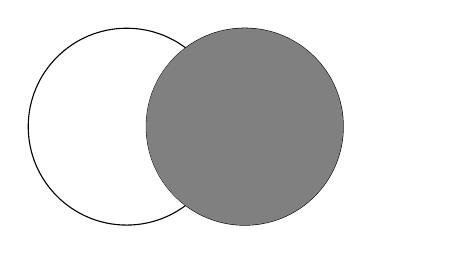
\begin{tikzpicture}
      \tikzset{circle node/.style={circle,draw=black, fill=none, minimum size=25mm, inner sep=0pt}}
      \node[circle node] (left) at (0,0) {};
      \node[circle node] (right) at (1.5,0) {};
      \begin{scope}
        \clip (0,-1.25) rectangle (4,1.25);
        \fill[gray] (1.5,0) circle (1.25cm);
      \end{scope}
      \begin{scope}
        \clip (1.5,0) circle (1.25cm);
        \fill[gray] (0,0) circle (1.25cm);
      \end{scope}
    \end{tikzpicture}
    \caption{\lstinline[style=sql]|RIGHT OUTER JOIN|}
  \end{subfigure}
  \hfill
  % FULL OUTER JOIN
  \begin{subfigure}[b]{0.45\textwidth}
    \centering
    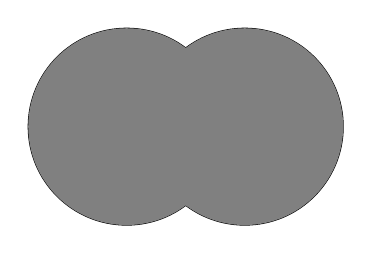
\begin{tikzpicture}
      \tikzset{circle node/.style={circle,draw=black, fill=none, minimum size=25mm, inner sep=0pt}}
      \node[circle node] (left) at (0,0) {};
      \node[circle node] (right) at (1.5,0) {};
      \fill[gray] (0,0) circle (1.25cm);
      \fill[gray] (1.5,0) circle (1.25cm);
    \end{tikzpicture}
    \caption{\lstinline[style=sql]|FULL OUTER JOIN|}
  \end{subfigure}
  \caption{Venn-Diagramme unterschiedlicher SQL-Joins}
  \label{fig:venn-joins}
\end{figure}


\subsection{\texorpdfstring{\lstinline[style=sql]|INNER JOIN| (=\lstinline[style=sql]|JOIN|)}{INNER JOIN (=JOIN)}}
Die Syntax eines \lstinline[style=sql]|INNER JOIN|-, oder auch einfach \lstinline[style=sql]|JOIN|-Befehls sieht wie folgt aus:

\begin{lstlisting}[style=sql]
SELECT kolonne1, kolonne2, ...
FROM tabelle1
INNER JOIN tabelle2
ON tabelle1.kolonne_id1 = tabelle2.kolonne_id2
\end{lstlisting}
Hier verbinden wir zwei Tabellen, indem wir zwei Kolonnen \texttt{kolonne\_id1} und \texttt{kolonne\_id2}, die derselben Information entsprechen (beispielsweise die user-ID), miteinander abgleichen. Beim \lstinline[style=sql]|INNER JOIN| werden nur die Zeilen aus \texttt{tabelle1} retourniert, für die es einen entsprechenden Wert in \texttt{kolonne\_id2} in \texttt{tabelle2} gibt. Alle Werte in \texttt{tabelle1} die mit keinem Wert in \texttt{tabelle2} überschneiden, sowie umgekehrt, tauchen nicht im Resultat auf (s. \cref{fig:venn-join}).

\begin{figure}[H]
  \centering
  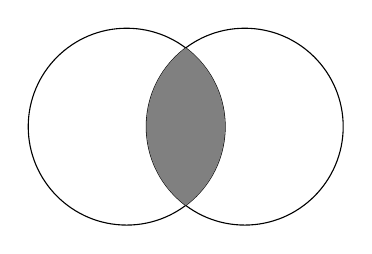
\begin{tikzpicture}
    \tikzset{circle node/.style={circle,draw=black, fill=none, minimum size=25mm, inner sep=0pt}}
    \node[circle node] (left) at (0,0) {};
    \node[circle node] (right) at (1.5,0) {};
    \begin{scope}
      \clip (0,0) circle (1.25cm);
      \fill[gray] (1.5,0) circle (1.25cm);
    \end{scope}
  \end{tikzpicture}
  \caption{\lstinline[style=sql]|(INNER) JOIN|}
  \label{fig:venn-join}
\end{figure}

Wichtig zu wissen ist zudem, dass \texttt{kolonne1, kolonne2} usw. auf der ersten Zeile nun sowohl von \texttt{tabelle1} wie auch \texttt{tabelle2} stammen können.

\begin{myexample}
Folgender Code gibt die ids aller user zurück, denen der user Mika Kaufmann folgt:
\begin{lstlisting}[style=sql]
SELECT follows.following_id, follows.follower_id, users.name 
FROM follows JOIN users 
ON follows.follower_id = users.id 
WHERE name="Mika Kaufmann"
\end{lstlisting}

Wie Sie sehen, kann es hilfreich sein, im \lstinline[style=sql]|SELECT|-Ausdruck explizit die Tabelle zu nennen, von welcher eine bestimmt Kolonne stammt.
\end{myexample}

Auch alle anderen SQL-Befehle wie beispielsweise \lstinline[style=sql]|GROUP BY| können nach einem \lstinline[style=sql]|JOIN|-Befehl verwendet werden.

\begin{myexample}\label{myexample:join-group}
Folgender Code gibt die Anzahl Fotos für alle Benutzer aus (und sortiert die Resultate absteigend):
\begin{lstlisting}[style=sql]
SELECT name, COUNT(*) AS "Anzahl Fotos"
FROM users
JOIN photos ON users.id = photos.user_id
GROUP BY user_id
ORDER BY `Anzahl Fotos` DESC
\end{lstlisting}
\end{myexample}

\begin{mycaution}
  Wie Sie in \cref{myexample:join-group} sehen, können Kolonnen jederzeit mit dem Befehl \lstinline[style=sql]|AS "Neuer Name"| umbenannt werden. Allerdings gilt es zu beachten, dass Abstände im Namen eher ungünstig sind: Falls der Name später wiederverwendet wird, wie etwa in einem \lstinline[style=sql]|ORDER BY|-Ausdruck, müssen sogenannte \textit{backticks} (\lstinline[style=sql]|`|) vor und nach dem Namen gesetzt werden.
\end{mycaution}

\begin{myexercise}
  Geben Sie die \texttt{id} aller Fotos in der Tabelle \texttt{likes} an, die der user Mika Kaufmann gelikt hat.
  \begin{myanswer}
    \begin{lstlisting}[style=sql]
SELECT photo_id, user_id, name 
FROM likes 
INNER JOIN users 
ON likes.user_id=users.id 
WHERE name="Mika Kaufmann"
\end{lstlisting}
  \end{myanswer}
\end{myexercise}
\begin{mychallenge}
  Challenge: Erstellen Sie eine Liste, wo für jedes Hamburger Mitglied die Anzahl seiner Fotos aufgeführt ist. Die Liste soll in absteigender Reihenfolge die Anzahl Fotos pro Mitglieder auflisten.
  \begin{myanswer}
    \begin{lstlisting}[style=sql]
SELECT city, username, COUNT(*) AS "Anzahl Fotos" 
FROM photos 
JOIN users ON photos.user_id = users.id 
WHERE city="Hamburg" 
GROUP BY username 
ORDER BY `Anzahl Fotos` DESC
\end{lstlisting}
  \end{myanswer}
\end{mychallenge}

\begin{myexercise}
  Es soll Werbung an alle Strandurlauber verschickt werden. Finden Sie alle Photos die den Hashtag \texttt{meer} enthalten. Geben Sie den Namen, die Emailadresse, den Geburtstag und die Stadt der zugehörigen Benutzer aus.
  \begin{myanswer}
    \begin{lstlisting}[style=sql]
SELECT description, name, email, birthday, city  
FROM photos 
JOIN users on photos.user_id = users.id 
WHERE description LIKE "%#meer%"
\end{lstlisting}
  \end{myanswer}
\end{myexercise}

\begin{mysubmission}
  Geben Sie die 5 User mit den meisten Followern aus.
  \begin{myanswer}
    \begin{lstlisting}[style=sql]
SELECT name, COUNT(*) AS "Followers"
FROM users JOIN follows on follows.following_id = users.id 
GROUP BY name
ORDER BY Followers DESC
LIMIT 5
\end{lstlisting}
  \end{myanswer}
\end{mysubmission}

\begin{mychallenge}
  Finden Sie heraus, welche 5 Fotos am meisten Likes erhalten haben. Geben Sie den Benutzernamen und Namen der Ersteller der Fotos an, die id der Fotos sowie die Anzahl Likes.
  \begin{myanswer}
    \begin{lstlisting}[style=sql]
SELECT users.username, users.name AS "Name", photos.id AS "Photo id", COUNT(likes.photo_id) AS "Likes"
FROM users
JOIN photos ON photos.user_id = users.id
JOIN likes ON photos.id = likes.photo_id
GROUP BY users.name, likes.photo_id
ORDER BY Likes DESC
LIMIT 5
\end{lstlisting}
  \end{myanswer}

\end{mychallenge}

\subsection{\texorpdfstring{\lstinline[style=sql]|LEFT JOIN| (=\lstinline[style=sql]|LEFT OUTER JOIN|)}{LEFT JOIN (=LEFT OUTER JOIN)}}
Ein \lstinline[style=sql]|LEFT JOIN|, oder \lstinline[style=sql]|LEFT OUTER JOIN| unterscheidet sich von einem \lstinline[style=sql]|INNER JOIN| dadurch, dass \textbf{alle} Einträge der ersten Tabelle (nach dem \lstinline[style=sql]|SELECT|-Befehl) in der neuen Tabelle erscheinen. Werte aus der zweiten Tabelle, die nicht in der ersten sind, werden jedoch nicht angezeigt (s. \cref{fig:venn-left-join}).

\begin{figure}[H]
  \centering
  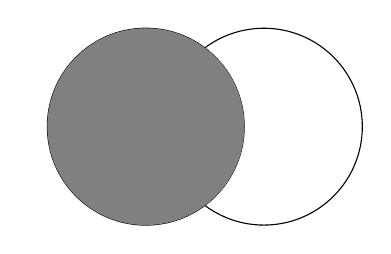
\begin{tikzpicture}
    \tikzset{circle node/.style={circle,draw=black, fill=none, minimum size=25mm, inner sep=0pt}}
    \node[circle node] (left) at (0,0) {};
    \node[circle node] (right) at (1.5,0) {};
    \begin{scope}
      \clip (-1.5,-1.25) rectangle (1.25,1.25);
      \fill[gray] (0,0) circle (1.25cm);
    \end{scope}
    \begin{scope}
      \clip (0,0) circle (1.25cm);
      \fill[gray] (1.5,0) circle (1.25cm);
    \end{scope}
  \end{tikzpicture}
  \caption{\lstinline[style=sql]|LEFT (OUTER) JOIN|}
  \label{fig:venn-left-join}
\end{figure}

\begin{myexercise}
  Diejenigen BenutzerInnen, die noch keine Fotos hochgeladen habe, sollen per Email dazu aufgefordert werden, Fotos hochzuladen. Finden Sie alle users, die noch keine Fotos hochgeladen haben. Geben Sie deren Name und Email-Adresse aus. Verwenden Sie statt \lstinline[style=sql]|WHERE| den Befehl \lstinline[style=sql]|HAVING|.
  \begin{myanswer}
    \begin{lstlisting}[style=sql]
SELECT users.name, users.email, COUNT(photos.id) AS "Anzahl Fotos"
FROM users
LEFT JOIN photos ON photos.user_id = users.id
GROUP BY users.name
HAVING `Anzahl Fotos` = 0
\end{lstlisting}
  \end{myanswer}
\end{myexercise}

\subsection{\texorpdfstring{\lstinline[style=sql]|RIGHT JOIN| (=\lstinline[style=sql]|RIGHT OUTER JOIN|)}{RIGHT JOIN (=RIGHT OUTER JOIN)}}
Ein \lstinline[style=sql]|RIGHT JOIN| funktioniert analog zu einem \lstinline[style=sql]|LEFT JOIN| (s. \cref{fig:venn-right-join}).

\begin{figure}[H]
  \centering
  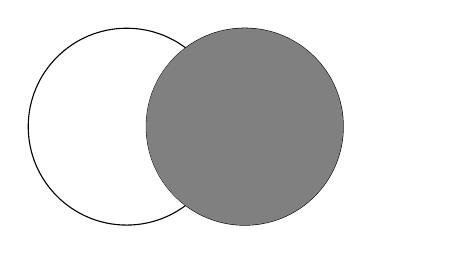
\begin{tikzpicture}
    \tikzset{circle node/.style={circle,draw=black, fill=none, minimum size=25mm, inner sep=0pt}}
    \node[circle node] (left) at (0,0) {};
    \node[circle node] (right) at (1.5,0) {};
    \begin{scope}
      \clip (0,-1.25) rectangle (4,1.25);
      \fill[gray] (1.5,0) circle (1.25cm);
    \end{scope}
    \begin{scope}
      \clip (1.5,0) circle (1.25cm);
      \fill[gray] (0,0) circle (1.25cm);
    \end{scope}
  \end{tikzpicture}
  \caption{\lstinline[style=sql]|RIGHT (OUTER) JOIN|}
  \label{fig:venn-right-join}
\end{figure}


\subsection{\texorpdfstring{\lstinline[style=sql]|FULL JOIN| (=\lstinline[style=sql]|FULL OUTER JOIN|)}{FULL JOIN (=FULL OUTER JOIN)}}
Bei einem \lstinline[style=sql]|FULL (OUTER) JOIN| werden alle Werte aus der ersten und der zweiten Tabelle angezeigt (s. \cref{fig:venn-outer-join}).

\begin{figure}[H]
  \centering
  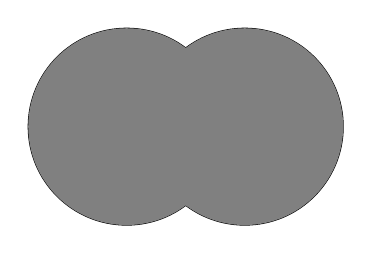
\begin{tikzpicture}
    \tikzset{circle node/.style={circle,draw=black, fill=none, minimum size=25mm, inner sep=0pt}}
    \node[circle node] (left) at (0,0) {};
    \node[circle node] (right) at (1.5,0) {};
    \fill[gray] (0,0) circle (1.25cm);
    \fill[gray] (1.5,0) circle (1.25cm);
  \end{tikzpicture}
  \caption{\lstinline[style=sql]|FULL (OUTER) JOIN|}
  \label{fig:venn-outer-join}
\end{figure}
In InstaHub funktioniert der \lstinline[style=sql]|FULL (OUTER) JOIN| nicht, weshalb es an dieser Stelle keine Übungen hierzu gibt.
